%-----------------------------------------------------------------------
% Cgcns: Compressible Navier Stokes Solver
%        REFERENCE MANUAL
%-----------------------------------------------------------------------
\documentclass{article}
% \usepackage[bookmarks=true]{hyperref} 
\usepackage[bookmarks=true,colorlinks=true,linkcolor=blue]{hyperref}

% \documentclass[11pt]{article}
% \usepackage[bookmarks=true]{hyperref} % this changes the page location!

% \input documentationPageSize.tex
\hbadness=10000 
\sloppy \hfuzz=30pt

\usepackage{calc}
\usepackage[lmargin=.75in,rmargin=.75in,tmargin=.75in,bmargin=.75in]{geometry}

% Remove bibliography heading
%% \input{bibent}
\usepackage{bibunits}

% \voffset=-.25truein
% \hoffset=-1.25truein
% \setlength{\textwidth}{7in}      % page width
% \setlength{\textheight}{9.5in}    % page height

\input homeHenshaw

% \input{pstricks}\input{pst-node}
% \input{colours}

\usepackage{amsmath}
\usepackage{amssymb}

\usepackage{verbatim}
\usepackage{moreverb}

\usepackage{graphics}    
\usepackage{epsfig}    
\usepackage{calc}
\usepackage{ifthen}
\usepackage{float}
% the next one cause the table of contents to disappear!
% * \usepackage{fancybox}

\usepackage{makeidx} % index
\makeindex
\newcommand{\Index}[1]{#1\index{#1}}

\usepackage{tikz}
\input trimFig.tex

% ---- we have lemmas and theorems in this paper ----
\newtheorem{assumption}{Assumption}
\newtheorem{definition}{Definition}


% \newcommand{\obFigures}{../docFigures}  % note: local version for OverBlown
\newcommand{\obFigures}{\homeHenshaw/res/OverBlown/docFigures}  % note: local version for OverBlown
\newcommand{\Overture}{{\bf Over\-ture\ }}
\newcommand{\OverBlown}{{\bf Over\-Blown\ }}
\newcommand{\OverBlownINS}{{\bf Over\-Blown\-INS\ }}
\newcommand{\OverBlownCNS}{{\bf Over\-Blown\-CNS\ }}
\newcommand{\overBlown}{{\bf over\-Blown\ }}

\newcommand{\obDir}{\homeHenshaw/res/OverBlown}
\newcommand{\ogenDir}{\homeHenshaw/Overture/ogen}
\newcommand{\cnsDocDir}{\homeHenshaw/cgDoc/cns}

% *** See http://www.eng.cam.ac.uk/help/tpl/textprocessing/squeeze.html
% By default, LaTeX doesn't like to fill more than 0.7 of a text page with tables and graphics, nor does it like too many figures per page. This behaviour can be changed by placing lines like the following before \begin{document}

\renewcommand\floatpagefraction{.9}
\renewcommand\topfraction{.9}
\renewcommand\bottomfraction{.9}
\renewcommand\textfraction{.1}   
\setcounter{totalnumber}{50}
\setcounter{topnumber}{50}
\setcounter{bottomnumber}{50}

% ===========================================================================================================
\begin{document}

\input wdhDefinitions.tex

\def\comma  {~~~,~~}
\newcommand{\uvd}{\mathbf{U}}
\def\ud     {{    U}}
\def\pd     {{    P}}
\def\calo{{\cal O}}

\newcommand{\mbar}{\bar{m}}
\newcommand{\Rbar}{\bar{R}}
\newcommand{\Ru}{R_u}         % universal gas constant
% \newcommand{\Iv}{{\bf I}}
% \newcommand{\qv}{{\bf q}}
\newcommand{\Div}{\grad\cdot}
\newcommand{\tauv}{\boldsymbol{\tau}}
\newcommand{\thetav}{\boldsymbol{\theta}}
% \newcommand{\omegav}{\mathbf{\omega}}
% \newcommand{\Omegav}{\mathbf{\Omega}}

\newcommand{\Omegav}{\boldsymbol{\Omega}}
\newcommand{\omegav}{\boldsymbol{\omega}}
\newcommand{\cm}{{\rm cm}}

\newcommand{\sumi}{\sum_{i=1}^n}
% \newcommand{\half}{{1\over2}}
\newcommand{\dt}{{\Delta t}}

\def\ff {\tt} % font for fortran variables
\newcommand{\Ic}{{\mathcal I}}
\newcommand{\Rc}{{\mathcal R}}
\newcommand{\Gc}{{\mathcal G}}


\vspace{5\baselineskip}
\begin{flushleft}
{\Large
{\bf Cgcns} Reference Manual: An Overture Solver for the Compressible Navier--Stokes Equations 
  on Composite Overlapping Grids \\
}
\vspace{2\baselineskip}
William D. Henshaw  \\
Centre for Applied Scientific Computing  \\
Lawrence Livermore National Laboratory      \\
Livermore, CA, 94551.  \\
% henshaw@llnl.gov \\
% http://www.llnl.gov/casc/people/henshaw \\
% http://www.llnl.gov/casc/Overture\\
\vspace{\baselineskip}
\today\\
\vspace{\baselineskip}
% UCRL-MA-134289

\vspace{4\baselineskip}

\noindent{\bf\large Abstract:}

{\bf Cgcns} can be used 
to solve the compressible Navier-Stokes equations, the reactive Euler equations,
multi-fluid and multi-phase equations on moving overlapping grids with
adaptive mesh refinement.
This document is a reference manual for Cgcns and
describes the governing equations, equations of state, reactions,
and boundary conditions. Also included are the results from a 
collection of computations that demonstrate the capabilities of Cgcns.



\end{flushleft}

\clearpage
\tableofcontents
% \listoffigures

\vfill\eject


% ----------------------------------------------------------------------------------------------
\section{Introduction}


Cgcns solves the compressible Navier-Stokes equations and reactive Euler (i.e. inviscid) equations
(and variations thereof, see below)
on overlapping grids and is built upon the \Overture 
framework~\cite{Brown97},\cite{Henshaw96a},\cite{iscope97}. 

Cgcns can be used to solve problems in complex geometry and moving and deforming
geometry. Cgcns uses adaptive mesh refinement (AMR).

Cgcns can be used to solve the
\begin{enumerate}
   \item Euler equations.
   \item reactive Euler equations with
      \begin{enumerate}
         \item one-step reaction~\ref{sec:oneStepReaction}
         \item ignition and growth reaction for explosives modeling~\ref{sec:ignitionAndGrowth}.
      \end{enumerate}
    \item compressible Navier-Stokes.
    \item multi-fluid Euler equations~\ref{sec:multifluid}.
    \item multi-phase Euler equations~\ref{sec:multiphase}.
\end{enumerate}

Here are some papers that describe the algorithms 
\begin{bibunit}[unsrt] % [siam]
\nocite{lrb2012a,mprxn2009,pog2008a,mfjwl2006,mog2006,reactamr2003b}
\putbib[\homeHenshaw/papers/henshaw]
\end{bibunit}

Here are some papers that use Cgcns to solve problems
\begin{bibunit}[unsrt] % [siam]
\nocite{hybridMultiphase2012a,fsi2012,OzlemSchwendemanKapilaHenshaw2012,SchwendemanKapilaHenshawLeeds2012,mprxn2009,fct2009,kapila2006,eliasson2007,mfrxn2007,mfjwl2006,ReedFriedHenshawTarver2006}
\putbib[\homeHenshaw/papers/henshaw]
\end{bibunit}

%\begin{bibunit}[unsrt] % [siam]
%\nocite{hybridMultiphase2012a,lrb2012a,fsi2012,OzlemSchwendemanKapilaHenshaw2012,SchwendemanKapilaHenshawLeeds2012,mprxn2009,fct2009,pog2008a,kapila2006,eliasson2007,mfrxn2007,mfjwl2006,ReedFriedHenshawTarver2006,mog2006,reactamr2003b}
%\putbib[\homeHenshaw/papers/henshaw]
%\end{bibunit}

% ----------------------------------------------------------------------------------------------
\section{The Equations}

\subsection{The compressible Euler equations} \label{sec:compressibleEuler}



\subsection{The compressible Navier-Stokes equations} \label{sec:compressibleNS}

The compressible Navier-Stokes equations can be written in
conservation form
$$
   \uv_t + {\partial \Fv\over \partial x_1}
         + {\partial \Gv\over \partial x_2}
         + {\partial \Hv\over \partial x_3}    =  0 .
$$
The vector of conserved variables $\uv$ is
$$
 \uv = \left[ \begin{array}{c}
    \rho \\ E \\ \rho v_1 \\ \rho v_2  \\  \rho v_3
              \end{array}\right]  ~,~
$$
where $\rho$, $E$ and $\vv=[v_1,v_2,v_3]^T$ denote the density, energy and
velocity vector with components parallel to the $x_1$, $x_2$, and $x_3$ axes, respectively.  The fluxes
$$
  \left[ \begin{array}{c}
    \Fv \\ \Gv \\ \Hv
              \end{array}\right]
 =\left[ \begin{array}{c}
    \Fv^C \\ \Gv^C \\ \Hv^C
              \end{array}\right]
 -\left[ \begin{array}{c}
    \Fv^V \\ \Gv^V \\ \Hv^V
              \end{array}\right]
$$
 are a combination of
{\it convective} fluxes $[\Fv^C,\Gv^C,\Hv^C]^T$ and {\it viscous}
fluxes $[\Fv^V,\Gv^V,\Hv^V]^T$.
% $[\Fv,\Gv,\Hv]=[\Fv^C-\Fv^V,\Gv^C-\Gv^V,\Hv^C-\Hv^V]$
The convective (or Euler) fluxes are given by
$$
 \Fv^C = \left[ \begin{array}{c}
 \rho v_1 \\ v_1(E+p) \\ \rho v_1^2 + p \\ \rho v_2 v_1 \\ \rho v_3 v_1
                \end{array}\right]  ~,~
 \Gv^C = \left[ \begin{array}{c}
 \rho v_2 \\ v_2(E+p) \\ \rho v_1 v_2 \\ \rho v_2^2+p \\ \rho v_3 v_2
                \end{array}\right]  ~,~
 \Hv^C = \left[ \begin{array}{c}
 \rho v_3 \\ v_3(E+p) \\ \rho v_1 v_3 \\ \rho v_2 v_3 \\ \rho v_3^2+p
                \end{array}\right]  ~,~
$$
and the viscous fluxes are
$$
 \Fv^V = \left[ \begin{array}{c}
    0 \\ \sum_n v_n\tau_{1n}-q_1
      \\ \tau_{11} \\  \tau_{12} \\ \tau_{13}
                \end{array}\right]  ~,~
 \Gv^V = \left[ \begin{array}{c}
    0 \\ \sum_n v_n\tau_{2n}-q_2
      \\ \tau_{21} \\  \tau_{22} \\ \tau_{23}
                \end{array}\right] ~,~
 \Hv^V = \left[ \begin{array}{c}
    0 \\ \sum_n v_n\tau_{3n}-q_3
      \\ \tau_{31} \\  \tau_{32} \\ \tau_{33}
                \end{array}\right]   ~.
$$
The pressure, p, and temperature, $T$, are given by the relations
\begin{eqnarray*}
   p &=& (\gamma-1)[ E - {1\over2} \rho (v_1^2+v_2^2+v_3^2) ], \\
   T &=& {p\over\rho R_g},
\end{eqnarray*}
where $R_g$ is the gas constant.
The viscous stress terms, $\tau_{mn}$, and heat flux, $q_n$, are given by
\begin{eqnarray*}
  \tau_{mn} &=&  \mu( {\partial v_n \over\partial x_m}
                     +{\partial v_m \over\partial x_n}     )
            - {2\over3}\mu( \grad\cdot\vv ) \delta_{mn}, \\
   q_n &=& -k {\partial T \over \partial x_n}
  =   -{k\over R_g} {\partial \over \partial x_n}
      \left({p\over\rho}\right)
  := -{\tilde{k}} {\partial \over \partial x_n}
      \left({p\over\rho}\right),
\end{eqnarray*}
where $\delta_{mn}$ is the Kronecker delta and $\tilde{k}=k/R_g$
is a scaled thermal conductivity.

% --------------------------------------------------------------------------------------------------
\subsection{The reactive Euler Equations} \label{sec:Euler}


% --------------------------------------------------------------------------------------------------
\subsection{The multi-fluid equations} \label{sec:multifluid}


% --------------------------------------------------------------------------------------------------
\subsection{The compressible multi-phase equations} \label{sec:multiphase}




% --------------------------------------------------------------------------------------------------
\section{Reactions}
\newcommand{\sigmat}{\tilde{\sigma}}

The species equation is
\[
   (\rho \Yv )_t + \grad\cdot( \rho \uv \Yv ) = R
\]

% --------------------------------------------------------------------------------------------------
\subsection{One-step Reaction} \label{sec:oneStepReaction}

For the one-step reaction
\begin{align*}
   R &= (1-Y)\sigma \exp(\epsilon^{-1}(1-1/T)) \\
\end{align*}
where
\begin{align*}
  \sigma &= { \sigmat \epsilon \over (\gamma -1) | Q | } \\
  \sigmat &= \mbox{rate constant} \\
  \epsilon &= \mbox{reciprocal activation energy} \\
   Q &= \mbox{heat release}
\end{align*}
The parameters $\sigmat$, $Q$ and $\epsilon$ are assigned in the command file.

% --------------------------------------------------------------------------------------------------
\def\bs{{\mathbf Y}} % {{\mathbf \xi}}
\subsection{Chain-branching reaction} \label{sec:chainBranchingReaction}

The chain-branching reaction is a three-step reaction given by
\[
\begin{array}{rcll}
{\cal F}&\buildrel k_I\over\longrightarrow&{\cal Y}, & \qquad\hbox{initiation,}\smallskip\\
{\cal F}+{\cal Y}&\buildrel k_B\over\longrightarrow&2{\cal Y}, & \qquad\hbox{branching,}\smallskip\\
{\cal Y}&\buildrel k_C\over\longrightarrow&{\cal P},  & \qquad\hbox{completion,}
\end{array}
\]
where ${\cal F}$, ${\cal Y}$ and ${\cal P}$ denote fuel, radical and product
species, respectively, and $k_I$, $k_B$ and $k_C$ are the rates of the
initiation, branching and completion reactions, respectively (see
\cite{ShortKapilaQuirk99}).  The initiation and branching rates are assumed to have
state-sensitive Arrhenius forms
\begin{equation}
k_i=\exp\left[{1\over\epsilon_i}\left({1\over T_i}-{1\over T}\right)\right],
\qquad\hbox{$i=I$ or $B$,}
\label{eq:chainBranchingRates}
\end{equation}
where $\epsilon_I$ and $\epsilon_B$ are reciprocal activation energies and $T_I$
and $T_B$ are cross-over temperatures.  The completion reaction rate is taken to
be $k_C=1$ which specifies the time scale.  For this case, $\bs=[\ss_1,\ss_2]^T$, 
where $\ss_1$ is the fraction of product and $\ss_2$ is the fraction of radical
(the fraction of fuel is $1-\ss_1-\ss_2$).  Laws of mass action give
\begin{equation}
\Rv = \left[
\begin{array}{c}
\ss_2k_C \\
(1-\ss_1-\ss_2)(k_I+\ss_2k_B)-\ss_2k_C
\end{array}\right],
\label{eq:chainBranching}
\end{equation}
and the contribution to the total energy is
\[
q=\ss_1Q_1+\ss_2Q_2.
\]
Here, $Q_1<0$ is the total chemical energy available in the unreacted mixture
and $Q_2>0$ is the amount of energy absorbed by the initiation and branching
reactions to convert fuel to (energetic) radical.


% --------------------------------------------------------------------------------------------------
\subsection{Ignition and growth reaction} \label{sec:ignitionAndGrowth}

Finish me.


% --------------------------------------------------------------------------------------------------
\subsection{Ignition and growth with desensitization} \label{sec:ignitionAndGrowthWithDesensitization}

Finish me.
% --------------------------------------------------------------------------------------------------
\subsection{One equation mixture fraction} \label{sec:oneEquationMixtureFraction}

Finish me.
% --------------------------------------------------------------------------------------------------
\subsection{Two equation mixture fraction and extent of reaction} \label{sec:twoEquationMixtureFraction}

Finish me.
% --------------------------------------------------------------------------------------------------
\subsection{One step pressure law} \label{sec:oneStepPressureLaw}

Finish me.




% ------------------------------------------------------------------------------------------------------------------------
\clearpage
\section{Axisymmetric Equations (Cylindrical Coordinates)}\label{sec:axisymmetricEquations}

The equations for axisymmetric flow are derived from the full Navier-Stokes equations written in
cylindrical coordinates $(x,r,\theta)$. Let $\vv = u \hat{\xv} + v \hat{\rv} + w\hat{\thetav}$
denote the components of the velocity in cylindrical coordinates (i.e. $u=V^x$, $v=V^r$ and $w=V^{\theta}$).
The Euler equations in conservation form in cylindrical coordinates are (*CHECK ME*) (finish me for Navier-Stokes)
\begin{align}
 & {\partial \rho\over\partial t} + {\partial \over\partial x}( \rho u ) + \frac{1}{r}{\partial \over\partial r}( r \rho v ) 
               + \frac{1}{r}{\partial \over\partial \theta}(\rho w) = 0\\
 &  {\partial \over\partial t}(\rho u)  + {\partial \over\partial x}( \rho u u ) + \frac{1}{r}{\partial \over\partial r}( r \rho v u ) 
               + \frac{1}{r}{\partial \over\partial \theta}(\rho w u) + {\partial p \over\partial x} = 0 \\ 
 &  {\partial \over\partial t}(\rho v) + {\partial \over\partial x}( \rho u v ) + \frac{1}{r}{\partial \over\partial r}( r \rho v v ) 
               + \frac{1}{r}{\partial \over\partial \theta}(\rho w v) + {\partial p \over\partial r} = 0 \\ 
 &  {\partial\over\partial t}(\rho w)  + {\partial \over\partial x}( \rho u w ) + \frac{1}{r}{\partial \over\partial r}( r \rho v w ) 
               + \frac{1}{r}{\partial \over\partial \theta}(\rho w w) + \frac{1}{r}{\partial p \over\partial \theta } = 0 \\ 
 &  {\partial\over\partial t}(E)  + {\partial \over\partial x}( u (E+p) ) + \frac{1}{r}{\partial \over\partial r}( r v (E+p) ) 
               + \frac{1}{r}{\partial \over\partial \theta}(w (E+p))  = 0
\end{align}
In the case where there is no variation in the angular direction $\theta$
direction we have the equations for two-dimensional axisymmetric flow, 
\begin{align}
 & {\partial \rho\over\partial t} + {\partial \over\partial x}( \rho u ) + \frac{1}{r}{\partial \over\partial r}( r \rho v ) 
               = 0\\
 &  {\partial \over\partial t}(\rho u)  + {\partial \over\partial x}( \rho u u ) + \frac{1}{r}{\partial \over\partial r}( r \rho v u ) 
                + {\partial p \over\partial x} = 0 \\ 
 &  {\partial \over\partial t}(\rho v) + {\partial \over\partial x}( \rho u v ) + \frac{1}{r}{\partial \over\partial r}( r \rho v v ) 
                + {\partial p \over\partial r} = 0 \\ 
 &  {\partial\over\partial t}(E)  + {\partial \over\partial x}( u (E+p) ) + \frac{1}{r}{\partial \over\partial r}( r v (E+p) ) 
                 = 0
\end{align}
The two-dimensional axisymmetric equations can be written in the form of the two-dimensional Cartesian equations plus source
terms
\begin{align}
 & {\partial \rho\over\partial t} + {\partial \over\partial x}( \rho u ) + {\partial \over\partial r}(\rho v ) 
            +   \frac{\rho v}{r}   = 0\\
 &  {\partial \over\partial t}(\rho u)  + {\partial \over\partial x}( \rho u u ) + {\partial \over\partial r}(\rho v u ) 
            +  \frac{\rho v u}{r}   + {\partial p \over\partial x} = 0 \\ 
 &  {\partial \over\partial t}(\rho v) + {\partial \over\partial x}( \rho u v ) + {\partial \over\partial r}(\rho v v ) 
           +  \frac{\rho v v}{r}    + {\partial p \over\partial r} = 0 \\ 
 &  {\partial\over\partial t}(E)  + {\partial \over\partial x}( u (E+p) ) + {\partial \over\partial r}(v (E+p) ) 
            +  \frac{v (E+p)}{r}    = 0
\end{align}
Note that on the axis $r=0$, $v=0$ and thus
\begin{align}
    \frac{\rho v}{r} &= {\partial \over\partial r}(\rho v ) ~= \rho {\partial v \over\partial r}, \qquad \text{on $r=0$} \\
    \frac{\rho u v}{r} &= {\partial \over\partial r}(\rho u v ) ~= \rho u {\partial v \over\partial r}, \qquad \text{on $r=0$} \\
     \text{etc.} & 
\end{align}

When using Cgcns to compute axisymmetric flow, the $r$ direction corresponds to the $y-$axis and the axis of symmetry
is $y=0$. 

% --------------------------------------------------------------------------------------------------------------
\section{ Discretization}\index{discretization!compressible Navier-Stokes}

Finish me ...

% -----------------------------------------------------------------------------------------------------------------
\input cnsBoundaryConditions



% ---------------------------------------------------------------------
\clearpage
\section{Equations of State}

There are a number of equations of state available. 

Notes to developers:
To add a new equation of state change the files
\begin{enumerate}
  \item CnsParameters.\{h,C\} : add EOS enums and names, change getDerivedFunction to define p for plotting.
  \item setupPde.C - change EOS menu 
  \item eosdat.h - define EOS for fortran
  \item dudr2d.f - change getp2d
  \item consPrim.bf - define conservative to primitive conversion
  \item Cgcns.C - output EOS name for info. 
\end{enumerate}


% ------------------------------------------------------------------------------------------
\subsection{Ideal Gas law}

The ideal gas law is
\begin{align}
 \rho e & =  C_v T = p/(\gamma-1) \qquad\mbox{(caloric EOS)}\label{eq:IdealEOS1} \\
 p & = \rho R_g T               \qquad\mbox{(thermal EOS)}\label{eq:IdealEOS2}
\end{align}
For a non-reactive flow, the temperature only appears in the boundary conditions, since the 
boundary conditions are applied to the primitive variables $(\rho,\uv,T)$.

The Godunov solver needs to know some derivatives of $p=P(\rho,\rho e)$ :
\begin{align}
 \left.{\partial p \over \partial \rho}\right\vert_{\rho e =K} &= 0, \qquad
 \left.{\partial p \over \partial \rho e}\right\vert_{\rho=K} = \gamma-1 
\end{align}

% ------------------------------------------------------------------------------------------
\subsection{JWL Equation of State}

This section needs to be written. See the paper ??.

% -------------------------------------------------------------
\subsection{Stiffened Gas Equation of State}


The stiffened gas law is
\begin{align}
 \rho e & =  (p + \gamma p_\infty)/(\gamma-1) \qquad\mbox{(caloric EOS)}\label{eq:StiffenedGasEOS1} \\
 p & = \rho R_g T               \qquad\mbox{(thermal EOS)}\label{eq:StiffenedGasEOS2}
\end{align}
Here $p_\infty$ is a constant. 
The second equation~\eqref{eq:StiffenedGasEOS2} can be thought of as the definition for $T$.
% This implies
% \begin{align}
%  p &= (\gamma-1)\rho e - \gamma p_\infty
% \end{align}

The Godunov solver needs to know some derivatives of $p=P(\rho,\rho e)$ :
\begin{align}
 \left.{\partial p \over \partial \rho}\right\vert_{\rho e =K} &= 0, \qquad
 \left.{\partial p \over \partial \rho e}\right\vert_{\rho=K} = \gamma-1 
\end{align}


The stiffened gas law is sometimes used to model shocks in water, which is less compressible than air.
Water might be modeled using $p_\infty = 4921.15$ bar and $\gamma = 5.5$. 


% -------------------------------------------------------------
\subsection{Tait Equation of State}

The Tait equation of state is
\begin{align}
 { p + B \over P_0 + B} &= \Big(\frac{\rho}{\rho_0}\Big)^n \\
 e & =C_v (T-T_0)+e_0 ~~~\mbox{(is this right?)} \\
  T &\equiv p/(R_g T) ~~~\mbox{(is this right?)}
\end{align}
Here $n$, $B$, $P_0$, $e_0$ and $\rho_0$ are constants.

Since $p$ only depends on $\rho$, the energy equation is decoupled from the equations for $(\rho,\rho\uv)$.

The Godunov solver needs to know some derivatives of $p=P(\rho,\rho e)$ :
\begin{align}
 \left.{\partial p \over \partial \rho}\right\vert_{\rho e =K} &=  { n\rho^{n-1} \over \rho_0^n} ~(P_0 + B), \qquad
 \left.{\partial p \over \partial \rho e}\right\vert_{\rho=K} = 0
\end{align}

% (p+B)/(p_ref+B)=(rho/rho_ref)^N
% and
% e=C_v (T-T_ref)+e_ref

% I guess this mean that one get
% dp(r,e)/dr[r*e=K] = dp/dr-dp/de*e/r = (p_ref+B)N(rhorho_ref)^(N-1)
% dp(r,e)/d(r*e)[r=K] = (1/r)*dp/de = 0

The Tait equation of state is used to model shocks in water with $n$=?, ...


% \newcommand{\cpc}{\sigma_C}
\newcommand{\cpc}{\kappa}
\clearpage
\subsection{Mie-Gruneisen Equation of State}
\newcommand{\rhot}{{\tilde\rho}}

The Mie-Gruneisen Equation of State refers to a general class of equations of state that 
are applicable to high temperature solids, see for example,
Lemons and Lund\cite{LemonsLund1999}.

The form of the Mie-Gruneisen EOS taken here is 
\begin{align}
 e & =  C_v T + {1 \over \rho} E_c(\rho) \qquad\mbox{(caloric EOS)}\label{eq:MGeos1} \\
 p & = \rho \cpc R_g T + F(\rho)                \qquad\mbox{(thermal EOS)}\label{eq:MGeos2}
\end{align}
where $F(\rho)$ and $E_c(\rho)$ are some given functions of the density.  The ideal gas law would 
correspond to $F=0$ and $E_c=0$.
Here we have assumed that $C_p$ and $C_v$ are constant and related by $C_p = C_v + \cpc R_g$,
for some constant, $\cpc$,
\begin{align*}
   C_p &= C_v + \cpc R_g \\
  \gamma &= {C_p\over C_v} \\
   R_g &= {\gamma -1 \over \cpc } C_v 
\end{align*}
which

The functions $F$ and $E_c$ are taken as
\begin{align}
  F(\rho) &= \alpha (v-1) + \beta (v-1)^2 \\
          &= \alpha {(1-\rhot)\over\rhot} + \beta {(1-\rhot)^2 \over \rhot^2} \\
  E_c(\rho) & = -\Big( {\alpha\over2} {(v-1)^2 \over v} + {\beta\over3} { (v-1)^3\over v} \Big)  \\
     & = - \Big( {\alpha\over2} {(1-\rhot)^2 \over \rhot} + {\beta\over3} { (1-\rhot)^3\over \rhot^2}  \Big) \\
     v &:= \rho_0/\rho = V/V_0  \\
     V &= 1/\rho \\
    \rhot &:= \rho/\rho_0
\end{align}
where $\rho_0=1/V_0$ is some reference state for the density (or specific volume $V=1/\rho$).

Note that for high temperatures $C_v$ is almost constant, $C_v \approx 3 R_g$.

Since $C_v = {\cpc R_g/(\gamma-1)}$ it follows from (\ref{eq:MGeos1}) and (\ref{eq:MGeos2}) that 
the pressure is given by
\[
   p = {\mathcal P}(\rho,e) := (\gamma-1) \Big(\rho e  - E_c(\rho) \Big) + F(\rho)
\]
or using $E=\rho e + \half \rho |\uv|^2$ implies
\[
   p = {\mathcal P}(\rho,\uv,E) := (\gamma-1) \Big(E - \half \rho |\uv|^2  - E_c(\rho) \Big) + F(\rho)
\]

It follows that 
\begin{equation}
     e = {1\over(\gamma-1)\rho} \Big(p - F(\rho)\Big) +{1\over\rho} E_c(\rho)
\end{equation}

\newcommand{\Hc}{{\mathcal H}}
The enthalpy $h=e+p/\rho$ can be written as a function of $p$ and $\rho$,
\begin{align}
   h = \Hc(\rho,p) & = 
           {\gamma\over(\gamma-1)} {p\over\rho} - {1\over (\gamma-1)\rho} F(\rho) + {E_c(\rho)\over\rho},
                                    \qquad\mbox{(enthalpy, Mie-Gruneisen)}.    \label{eq:enthalpy} \\
        &=   {\gamma\over(\gamma-1)} {p\over\rho} + G(\rho) \\
  G(\rho) &:= - {1\over (\gamma-1)\rho} F(\rho) + {E_c(\rho)\over\rho}
\end{align}
% \begin{align*}
%    p &= F(\rho) + (\gamma-1)( E -\half \rho |\uv|^2 - E_c(\rho) ) \\
%      &= F(\rho) + (\gamma-1)( \rho e - E_c(\rho) ) \\ 
%      &= F(\rho) + (\gamma-1)( \rho C_v T )   \\
% \end{align*}
    
\noindent{\bf Speed of sound} Given a caloric EOS for the enthalpy of the form $h=\Hc(p,\rho)$ the
speed of sound is (see Toro~\cite{Toro97})
\[
        a^2 =  - { \partial_\rho \Hc \over \partial_p \Hc - \rho^{-1} }
\]
and thus
\begin{align*}
   a^2 &= { {\gamma\over(\gamma-1)} {p\over\rho^2} + G'(\rho)
             \over 
             {\gamma\over(\gamma-1)\rho} - \rho^{-1} } \\
   a^2  &= {\gamma p\over\rho} +  \rho(\gamma-1)G'(\rho)
\end{align*}

%\noindent{\bf Reactions} Suppose we have an Arhrenius reaction rate term of the form
%\[
%      A \exp(-E_A/( k T )
%\]
%This can 

% ------------------------------------------------------------------------------------------
\subsection{User defined equation of state} \label{sec:userDefinedEOS}

New equations of state can be created by changing the file {\tt cg/cns/src/userDefinedEOS.C}.

***FINISH ME***


% ------------------------------------------------------------------------------------------

\section{Shock Jump Conditions}

For the one-dimensional Euler equations, the jump conditions at a shock travelling with speed $U$
are (see for example Whitham~\cite{Whitham74})
\begin{align*}
          [\rho v] &= 0 \\
         [p+\rho v^2] &= 0   \\
         [h+ \half v^2] &= 0   
\end{align*}
here $v=U-u$ is the speed relative to the shock and $h=e+p/\rho$ is the enthalpy.

Written out in terms of the states on either side of the shock:
\begin{align*}
          \rho_2 v_2 &= \rho_1 v_1 \\
         p_2+\rho_2 v_2^2 &= p_1+\rho_1 v_1^2   \\
         h_1+\half v_1^2 &= h_2+\half v_2^2 
\end{align*}

Given state 1, $[\rho_1~ v_1~ h_1~ p_1]$,  state 2 can be determined by writing 
$v2$, $p_2$ as functions of $\rho_2$
\begin{align*}
  v_2 &= (\rho_1 v_1)/\rho_2 \\
  p_2 &= P(\rho_2) = (p_1+\rho_1 v_1^2) - (\rho_1 v_1)^2/\rho_2
\end{align*}

If $h=e+p/\rho$ can be written, using the equations of state, as a function of $\rho$ and $p$,
$h = \Hc(\rho,p)$ then we can form an equation
\begin{align*}
  \Hc(\rho_2,P(\rho_2)) + \half (\rho_1 v_1)^2/\rho_2^2 &= h_1^2 + \half v_1^2
\end{align*}
which defines a single equation of $\rho_2$ in terms of the known values of state 1. Thus this 
last equation can be hopefully solved 
for $\rho_2$. Given $\rho_2$ the other state 2 variables are easily computed from the relations
given above.

For the 
Mie-Gruneisen equation of state the enthalpy $h=\Hc(\rho,p)$ is given by equation~(\ref{eq:enthalpy}).

% Note that for an ideal gas
% \[
%   \H_c(\rho,p)={\gamma\over(\gamma-1)} {p\over\rho} \qquad\mbox{(enthalpy, Ideal Gas)}.
% \]
% while 
% 
% \[
%     p = F(\rho) + (\gamma-1)[ \rho e - E_c(\rho) ]
% \]
% and thus
%\[
%   H(\rho,p) = {\gamma\over(\gamma-1)} {p\over\rho} - {1\over (\gamma-1)\rho} F(\rho) + {E_c(\rho)\over\rho}
%        \qquad\mbox{(enthalpy, Mie-Gruneisen)}.
%\]

%\noindent {\bf Example:} Suppose that in non-dimensional units,
%the state in front of the shock is given by $\rho_1=1$, $u_1=0$, $E_1=1.75$ and suppose the shock velocity is $U=2$. 
%The for $\gamma=4/3$, $\alpha=\half$, $\beta=\half$ and $\rho_0=\rho_1$ the state behind the shock is
$\rho_2\approx 3.4058$, $u_2\approx 1.4128$, $p_2\approx 3.4089$ and $E_2\approx 14.1614$.
% from shock.maple:
% $a=.5; $b=.5; $v0=1.; $gamma=4./3.; 
% $r1=1.; $u1=0.; $E1=1.75; 
% $r2=3.40584; $u2=1.41277; $E2=14.16144; 

\clearpage
\section{Travelling Wave profiles for Reacting flow}\index{travelling waves}

Suppose that we look for a steady travelling wave profile of the form $f(x-Ut)$ then the
Euler equations for a one-dimensional reacting flow become
\begin{align*}
  - U \rho_x + (\rho u)_x &=0 \\
  -U (\rho u)_x + (\rho u^2 + p )_x &= 0 \\
  -U E_x + ( uE + pu)_x &=0   \\
  -U (\rho Y)_x + (\rho u Y)_x &= \rho R
\end{align*}
where
\begin{align*}
    e &= {1\over (\gamma-1)\rho} (p - F(\rho) ) + {1 \over \rho} E_c \\
    h &= {\gamma\over (\gamma-1)\rho} p  - {1\over (\gamma-1)\rho} (pF(\rho) ) + {1 \over \rho} E_c \\
    E &= {1\over (\gamma-1)} (p-F) + E_c + \rho Q Y \\
    T &= (p-F)/(\cpc \rho R_g)
\end{align*}

Letting $v=u-U$ it follows that 
\begin{align*}
  (\rho v)_x &=0 \\
  (\rho v^2 + p )_x &=0 \\
  (e + p/\rho + \half v^2 + Q Y )_x &=0 \\
   (\rho v Y)_x &= \rho R 
\end{align*}
Let $\rho_0$, $u_0$, $p_0$, etc. denote the solution values in the unreacted state and
letting $m=\rho v$ (constant) then
\begin{align*}
   p - p_0 &= m^2 ( \rho_0^{-1} - \rho^{-1} ) \qquad\mbox{(Rayleigh line)} \\
           & = m ( v_0 - v )  \\
   v - v_0 &= m( \rho_0^{-1} + \rho^{-1} ) \\
    v^2 - v_0^2 &= -(p - p_0)( \rho_0^{-1} + \rho^{-1} ) \\
   {\gamma\over (\gamma-1)} (p/\rho - p_0/\rho_0 ) &+ \half( v^2 - v_0^2) + Q(Y-Y_0) + G(\rho)-G(\rho_0) =0\\
   G(\rho) &\equiv - {1\over (\gamma-1)\rho} (F(\rho) ) + {1 \over \rho} E_c 
\end{align*}
and thus the Hugoniot for this system is 
\begin{align*}
  {\cal H}(p,\rho,Y) &\equiv 
      {\gamma\over (\gamma-1)} (p/\rho - p_0/\rho_0 ) -\half(p + p_0)( \rho_0^{-1} + \rho^{-1} ) 
           + Q(Y-Y_0) + G(\rho)-G(\rho_0) =0
\end{align*}
The Hugoniot only depends on the thermodynamic quantities and not the velocity.


\begin{figure}[hbt]
  \begin{center}
    \includegraphics[width=.75\linewidth]{\cnsDocDir/fig/Hugoniot}
  \end{center}
\caption{Hugoniot curves and Rayleigh line for the 1D reacting flow problem. The solution must always remain
  on the Rayleigh line. The Hugoniot curve moves upward to the right as $Y$ increases. The final state
   is found at the intersection of the Rayleigh line and the Hugoniot curve for $Y=1$. The Chapman-Joguet
detonation occurs when the Hugoniot curve for $Y=1$ is tangent to the Rayleigh line.} \label{fig:Hugoniot}
\end{figure}

%- \begin{figure}[hbt]
%-   \begin{center}
%-    \epsfig{file=\obDir/doc/Hugoniot.eps,width=.75\linewidth}
%-   \end{center}
%- \caption{Hugoniot curves and Rayleigh line for the 1D reacting flow problem. The solution must always remain
%-   on the Rayleigh line. The Hugoniot curve moves upward to the right as $Y$ increases. The final state
%-    is found at the intersection of the Rayleigh line and the Hugoniot curve for $Y=1$. The Chapman-Joguet
%- detonation occurs when the Hugoniot curve for $Y=1$ is tangent to the Rayleigh line.} \label{fig:Hugoniot}
%- \end{figure}

\newcommand{\vf}{V} % volume fraction 1/rho

For each fixed value of $Y$, $0 \le Y \le 1$ the intersection of the Rayleigh line and the Hugoniot
will determine a value of $\rho$:
\begin{align*}
   p - p_0 &= m^2 ( \rho_0^{-1} - \rho^{-1} ) \qquad\mbox{(Rayleigh line)} \\
  {\gamma\over (\gamma-1)} (p/\rho - p_0/\rho_0 ) & -\half(p - p_0)( \rho_0^{-1} + \rho^{-1} ) 
           + Q(Y-Y_0) + G(\rho)-G(\rho_0) =0 \qquad\mbox{(Hugoniot)}
\end{align*}
or in terms of $\vf=1/\rho$, 
\begin{align*}
   p &= p_0 + m^2 ( \vf_0 - \vf ) \qquad\mbox{(Rayleigh line)} \\
   p &= { p_0 \big[ \Gamma \vf_0 - \vf \big] - 2\big[ Q(Y-Y_0) + G(\rho)-G(\rho_0) \big] \over
                 \Gamma\vf -\vf_0 }  \qquad\mbox{(Hugoniot)} \\
  \Gamma &= {\gamma+1 \over \gamma -1} 
\end{align*}

We can thus determine $\rho$ as a function of $Y$. It follows that we also know $v$, $p$, $T$ etc. as a function
of $Y$ since these are known as functions of $\rho$,

For the one-step reaction
\begin{align*}
   R &= (1-Y)\sigma \exp(\epsilon^{-1}(1-1/T)) \\
\end{align*}
and thus
\begin{align*}
  Y_x &= {\rho\over m} (1-Y)\sigma \exp(\epsilon^{-1}(1-1/T)) \\
      &\equiv {\mathcal R}(Y)
\end{align*}
This last equation can be integrated as an initial value problem 
to give $Y=Y(x)$. Alternatively since $Y$ is a monotone function 
we can instead solve
\begin{align*}
  {d x \over d Y} & = 1/{\mathcal R}(Y)
\end{align*}
by quadrature from some known point $Y(x_a)=Y_a$, to give $x$ as a single valued function
of $Y$
\begin{align*}
   x(Y) - x_a &= \int_{Y_a}^Y 1/{\mathcal R}(\xi) ~d\xi
\end{align*}

\begin{figure}[hbt]
 \begin{center}
   \includegraphics[width=.48\linewidth]{\cnsDocDir/fig/profileIdealOneStep}
   \includegraphics[width=.48\linewidth]{\cnsDocDir/fig/profileMieGruneisen}
 \end{center}
\caption{Profiles of a steady (Chapman-Jouget) detonation for an ideal gas (left) and
   the Mie-Gruneisen EOS (right). } \label{fig:detonationCJ}
\end{figure}

% \begin{figure}[hbt]
%   \begin{center}
%    \epsfig{file=\obDir/doc/profileIdealOneStep.eps,width=.49\linewidth}
%    \epsfig{file=\obDir/doc/profileMieGruneisen.eps,width=.49\linewidth}
%   \end{center}
% \caption{Profiles of a steady (Chapman-Jouget) detonation for an ideal gas (left) and
%    the Mie-Gruneisen EOS (right). } \label{fig:detonationCJ}
% \end{figure}

The condition for a Chapman-Jouget detonation is that the Rayleigh-line be tangent to the Hugoniot
which implies
\[
   \vf_{CJ} = \vf_0/\Gamma \pm 
    {1\over \Gamma m} \Big[ \vf_0\big( p_0 \Gamma^2 -1\big) -2 {\Gamma\over\vf_0} ( Q+G(\vf_{CG})) \Big]^{1/2}
\] 
This last equation relates the volume fraction of the final state, $V_{CJ}$ to the initial values
for $p_0$, $V_0$ and $m$. **** check this and finish ****

Figure~\ref{fig:detonationCJIdealComparison} compares a computed solution with the analytic solution
for the case of an ideal gas ($\alpha=0$, $\beta=0$).
\begin{figure}[hbt]
\begin{center}
  \includegraphics[width=.75\linewidth]{\cnsDocDir/fig/profileIdealvsComputedLevel2}
  \includegraphics[width=.75\linewidth]{\cnsDocDir/fig/profileIdealvsComputedLevel3}
 \end{center}
\caption{Comparison of the computed solution versus the analytic solution for a steady (Chapman-Jouget) detonation for an ideal gas. Left: 2-levels of AMR $r=4$. Right: 3-levels of AMR. } \label{fig:detonationCJIdealComparison}
\end{figure}


% \begin{figure}[hbt]
%   \begin{center}
%    \epsfig{file=\obDir/doc/profileIdealvsComputedLevel2.eps,width=.75\linewidth}
%    \epsfig{file=\obDir/doc/profileIdealvsComputedLevel3.eps,width=.75\linewidth}
%   \end{center}
% \caption{Comparison of the computed solution versus the analytic solution for a steady (Chapman-Jouget) detonation for an ideal gas. Left: 2-levels of AMR $r=4$. Right: 3-levels of AMR. } \label{fig:detonationCJIdealComparison}
% \end{figure}


% Figure~\ref{fig:detonationCJComparison} compares a computed solution with the analytic solution.
% \begin{figure}[hbt]
%   \begin{center}
%    \epsfig{file=\obDir/doc/profileMGvsComputedLevel2.eps,width=.75\linewidth}
%    \epsfig{file=\obDir/doc/profileMGvsComputedLevel3.eps,width=.75\linewidth}
%   \end{center}
% \caption{Comparison of the computed solution ($t=1$) versus the analytic solution for a steady (Chapman-Jouget) detonation for the Mie-Gruneisen EOS. Left: 2-levels of AMR $r=4$. Right: 3-levels of AMR. The
% base grid has $\Delta x = 5.e-3$ before refinements were added.} \label{fig:detonationCJComparison}
% \end{figure}

Figure~\ref{fig:detonationCJComparisonKappa1p5} compares a computed solution with the analytic solution for
a different case with $\kappa=3/2$.
\begin{figure}[hbt]
\begin{center}
  \includegraphics[width=.49\linewidth]{\cnsDocDir/fig/profileMGvsComputedKappa1p5Level2}
  \includegraphics[width=.49\linewidth]{\cnsDocDir/fig/profileMGvsComputedKappa1p5Level3}
 \end{center}
\caption{Comparison of the computed solution ($t=1$) versus the analytic solution for a steady (Chapman-Jouget) detonation for the Mie-Gruneisen EOS. Left: 2-levels of AMR $r=4$. Right: 3-levels of AMR. The
base grid has $\Delta x = 5.e-3$ before refinements were added.} \label{fig:detonationCJComparisonKappa1p5}
\end{figure}
% 
% \begin{figure}[hbt]
%   \begin{center}
%    \epsfig{file=\obDir/doc/profileMGvsComputedKappa1p5Level2.eps,width=.49\linewidth}
%    \epsfig{file=\obDir/doc/profileMGvsComputedKappa1p5Level3.eps,width=.49\linewidth}
%   \end{center}
% \caption{Comparison of the computed solution ($t=1$) versus the analytic solution for a steady (Chapman-Jouget) detonation for the Mie-Gruneisen EOS. Left: 2-levels of AMR $r=4$. Right: 3-levels of AMR. The
% base grid has $\Delta x = 5.e-3$ before refinements were added.} \label{fig:detonationCJComparisonKappa1p5}
% \end{figure}



\begin{figure}[hbt]
\begin{center}
  \includegraphics[width=.49\linewidth]{\cnsDocDir/fig/profileMGconserved}
  \includegraphics[width=.49\linewidth]{\cnsDocDir/fig/profileMGconervedComputed}
 \end{center}
\caption{Diagnostics of the solution. The error in some conserved quantities is shown for
   the analytic solution (left, note scale) and the computed solution (right). The case was for a 
    Mie-Gruneisen EOS (3-levels results shown in figure~\ref{fig:detonationCJComparisonKappa1p5}). } 
   \label{fig:detonationConserved}
\end{figure}

% \begin{figure}[hbt]
%   \begin{center}
%    \epsfig{file=\obDir/doc/profileMGconserved.eps,width=.49\linewidth}
%    \epsfig{file=\obDir/doc/profileMGconervedComputed.eps,width=.49\linewidth}
%   \end{center}
% \caption{Diagnostics of the solution. The error in some conserved quantities is shown for
%    the analytic solution (left, note scale) and the computed solution (right). The case was for a 
%     Mie-Gruneisen EOS (3-levels results shown in figure~\ref{fig:detonationCJComparisonKappa1p5}). } 
%    \label{fig:detonationConserved}
% \end{figure}
% 


\clearpage
\section{Convergence results}\index{convergence results!CNS}

% ==============================================================================================================
\clearpage
\input sampleSimulations

% Here is a collection of interesting examples computed with the Cgcns compressible solver.

% \subsection{Incompressible flow past a mast and sail}


% -------------------------------------------------------------------------------------------------
\vfill\eject
\bibliography{\homeHenshaw/papers/henshaw}
\bibliographystyle{siam}


\printindex


\end{document}
